\documentclass{article}


\usepackage[utf8]{inputenc}


\usepackage{tikz}
\usepackage[short,nodayofweek,level,12hr]{datetime} 


\usepackage{color}
\usepackage{amsmath}
\usepackage{amssymb}
\usepackage{amsthm}
\usepackage[
%  disable, %turn off todonotes
 colorinlistoftodos, %enable a coloured square in the list of todos
 textwidth=\marginparwidth, %set the width of the todonotes
 textsize=scriptsize, %size of the text in the todonotes
 ]{todonotes}

\usepackage[a4paper, total={6in, 10in}]{geometry}
\setlength\parindent{0in}

\usepackage[english]{babel}
\usepackage{datetime}
\usepackage{graphicx}
\definecolor{suchblue}{RGB}{150, 255, 150}
\usepackage{float}
\usepackage{caption}
\usepackage{mathtools}
\newtheorem{theorem}{Theorem}
\newtheorem{corollary}{Corollary}[section]
\newtheorem{lemma}[section]{Lemma}
\newtheorem*{remark}{Remark}
\newtheorem{definition}{Definition}[section]
\newtheorem{proposition}{Proposition}[section]


\usepackage{algorithm}% http://ctan.org/pkg/algorithms
\usepackage{algorithmic}% http://ctan.org/pkg/algorithms
\newcommand{\pluseq}{\mathrel{+}=}
\DeclareMathOperator{\Var}{Var}
\usepackage{color}
\usepackage{hyperref}
\usepackage{tipa}
\usepackage{pgfplots}
\pgfplotsset{compat = 1.16}
\usepackage{footmisc}
\usepackage{listings}
\usepackage{tcolorbox}
\usepackage{enumitem}

\usepackage{array}
\usepackage{lmodern,babel,adjustbox,booktabs,multirow}
\usepackage[normalem]{ulem}


\renewcommand{\thefootnote}{[\arabic{footnote}]}
\newcommand{\mbf}[1]{\mathbf{#1}}
\newcommand{\mbs}[1]{\boldsymbol{#1}}
\newcommand{\mR}{\mathbb{R}}
\newcommand{\mE}{\mathbb{E}}
\newcommand{\mC}{\mathbb{C}}
\newcommand{\mZ}{\mathbb{Z}}
\newcommand{\mN}{\mathbb{N}}
\newcommand{\Tr}[1]{\Text{Tr}{\left(#1}\right)}
\newcommand{\norm}[1]{\left\lVert#1\right\rVert}
\newcommand*{\cond}{\hspace*{1pt} |\hspace*{1pt}}

\newcommand{\tobi}[1]{\todo[color=suchblue!40,author=Tobias]{#1}}

\DeclareMathOperator*{\argmax}{arg\,max}
\DeclareMathOperator*{\argmin}{arg\,min}
\DeclareMathOperator*{\Cov}{Cov}
\DeclareMathOperator*{\logit}{logit}
\DeclareMathOperator*{\Std}{Std}

\lstdefinestyle{mystyle}{
  belowcaptionskip=1\baselineskip,
  breaklines=true,
  xleftmargin=\parindent,
  language=C,
  showstringspaces=false,
  basicstyle=\footnotesize\ttfamily,
  keywordstyle=\bfseries\color{green!40!black},
  commentstyle=\itshape\color{purple!40!black},
  identifierstyle=\color{blue},
  stringstyle=\color{orange},
  backgroundcolor = \color{white},
}
\lstdefinestyle{console}{
  belowcaptionskip=1\baselineskip,
  breaklines=true,
  xleftmargin=\parindent,
  language=C,
  showstringspaces=false,
  keywordstyle=\bfseries\color{white},
  commentstyle=\itshape\color{white},
  identifierstyle=\color{white},
  stringstyle=\color{white},
  numberstyle=\color{white},
  backgroundcolor=\color{black},
  basicstyle = \color{white}\footnotesize\ttfamily,
}
\lstset{style=mystyle,breaklines=true}

\newcommand\NoIndent[1]{%
  \par\vbox{\parbox[t]{\linewidth}{#1}}%
}


% define enviroments
\theoremstyle{definition}
\newtheorem{example}{Eksempel}[section]


\usepackage[backend=bibtex,
  bibencoding=utf8,
  sorting = nty, 
  ]{biblatex}



\addbibresource{mybib.bib}
\DeclareNameAlias{sortname}{last-first}
\DeclareNameAlias{default}{last-first}
\DefineBibliographyStrings{english}{%
   bibliography = {Bibliografi},
}	
\renewcommand*{\bibfont}{\small}



\title{Introduktion til Sandsynlighed og Statistik \\
til modellering og simulering  \\
\large Datalogi og Software 1. semester}


\date{Aalborg Universitet, \today}
\author{Tobias Kallehauge}


\begin{document}
\maketitle
\newpage
Denne note omhandler sandsynlighed, statistik og hvordan disse kan bruges i praksis specielt i sammenhæng med simuleringer, hvor det ofte er nødvendigt at udtrække tal fra bestemte sandsynlighedsfordelinger. Der vil primært fokuseres på den matematiske forståelse, men til sidst i noten gives et par eksempler på hvordan teorien kan bruges i et C-program. Formålet med noten er at give den \emph{nødvendige} teori til software- og datalogiprojekter på  1 semester, og teorien gennemgås derfor relativt overfladisk med kun få eksempler. Den primære kilde bag noten er \cite{olofsson2012}, som er gratis tilgængelig på \href{aub.aau.dk}{aub.aau.dk}. Heri findes også beviser for resultaterne, der er udeladt i noten. Forslag til ændringer, stavefejl mm. kan sendes til \href{mailto:tkal@es.aau.dk}{tkal@es.aau.dk}. 
\section{Introduktion til sandsynlighed}
\emph{Sandsynlighed} er et begreb der (mis)bruges i mange sammenhænge indenfor videnskab, økonomi, politik, osv., men helt grundlæggende er det en matematisk konstruktion med en bestemt definition. For at måle sandsynlighed indføres sandsynlighedsmålet $P$, som er en funktion der bestemmer sandsynligheden for udfald i \emph{tilfældige eksperimenter}. Hvis et tilfældigt eksperiment har mulige udfald $A_1, A_2,\dots$ da vil $P(A_i)$ være sandsynligheden for netop udfaldet $A_i$.
\begin{example}
Vi kaster en fair 6-siddet terning med mulige udfald 
$$A_1 = \text{``slå en 1'er''}, \quad  A_2 = \text{``slå en 2'er''}, \quad \dots \quad, A_6 = \text{``slå en 6'er''}$$
Sandsynligheden for alle udfald er lige stor og vi har eksempelvis at \\
$P(A_6) = P(``\text{slå en 6'er}'') = 1/6 \approx 0.17\%$. 
\end{example}
Funktionen $P$ er defineret ud fra en række matematiske egenskaber, hvoraf den vigtigste er at den altid antager værdier mellem $0$ og $1$ (se den fulde definition i \cite[sektion 1.3]{olofsson2012}). 
\\ \\
For at formalisere notationen i tilfældige forsøg,  eksempelvis at slå med en terning, indfører vi begrebet \textit{tilfældige variable}. En tilfældig variabel er en funktion $X: S \to\mR$, der får sine værdier fra et tilfældigt forsøg hvor $S$ er mængden af mulige udfald. I forsøget med terningen vil $X(\text{slå en 6'er}) = 6$, $X(\text{slå en 1'er}) = 1$, osv. Vi kan så skrive $P(X = 6) = 1/6$. Et andet eksempel er møntkast hvor den tilfældige variabel $X$ kan repræsentere antallet af kroner i løbet af 3 møntkast. Hver vil $X(PPK) = 1$, $X(KKP) = 2$, $X(KKK) = 3$ osv.
\\ \\
Med begrebet tilfældige variable kan vi indføre \textit{sandsynlighedsmassefunktionen}, på engelsk \textit{probability mass funktion} (pmf), som egentlig blot er en nemmere notations metode. En pmf $p_X$ er defineret som $p_X(x) = P(X = x)$ for en tilfældig variable $X$. Bemærk her at $X$ er den tilfældige variabel mens $x$ er et reelt tal, eksempelvis er $P(\text{slå en 6'er}) = P(X = 6) = p_X(6)$. 

\section{Fordelinger og fordelingsfunktioner}
Før vi kan indføre fordelingsfunktioner skal vi kategorisere mellem \emph{diskrete} og \emph{kontinuerte} tilfældige variable. Eksemplerne vi har set indtil videre er diskrete da der er et \emph{tælleligt} antal udfald. Det også muligt at have en diskret variabel med tælleligt uendelig mange udfald så længe man kan associere associere udfaldene med en tællelig mængde såsom de ikke negative heltal $\{0,1,2,\dots\}$. Antallet af terningslag før der slås en 6'er et eksempel på en tællelig uendelig mænge da der ikke er en øvre grænse for antal slag. Kontinuerte tilfældige variable derimod er \textit{utællelige} og er typisk associeret med de reelle tal $\mR$ eller et interval heri. Eksempelvis er højden af en tilfældigt udvalgt person eller tiden det tager for et atom at udfalde radioaktivt begge kontinuerte tilfældig variable. 
\subsection{Diskrete fordelinger}
Vi indfører nu \emph{sandsynlighedsmassefunktionen}, på engelsk \textit{probability mass funktion} (pmf). En pmf $p_X$ er defineret som $p_X(x) = P(X = x)$ for en tilfældig variable $X$. Bemærk her at $X$ er den tilfældige variabel mens $x$ er et reelt tal.
\begin{example} \label{ex:terning3} I $X$ fra eksempel \ref{ex:terning2} med terningkast er $p_X(x) = 1/6$ for $x = 1,2,\dots, 6$ og vi har eksempelvis $P(\text{``slå en 6'er''}) = P(X = 6) = p_X(6) = 1/6$. 
\end{example}
\begin{example} \label{ex:terning4} For en tilfældig variabel $X$ har vi givet pmf'en:
\begin{align*}
p_X(x) = \begin{cases}
\frac{3}{6} & x = -1 \\
\frac{1}{6} & x = 0 \\ 
\frac{2}{6} & x = 1
\end{cases},
\end{align*}
og vi har eksempelvis at $P(X = 0) = p_X(0) = \frac{1}{6}$. Selvom vi ikke ved noget om hvilket tilfældigt forsøg $X$ stammer fra, ved vi ud fra $p_X$ alt om hvordan $X$ opfører sig fra et statistisk synspunkt. Vi siger derfor at $p_X$ karakteriserer $X$ fuldstændigt samt at $X$ følger fordelingen for $p_X$. 
\end{example}
Med en pmf kan man nemt lave beregninger, der omhandler delmængder af udfaldsrummet. 
\begin{example}
Givet pmf'en for $X$ i eksempel \ref{ex:terning3} med terningkast har vi eksempelvis:
\begin{align*}
P(\text{``Slå mindst 3''}) &= P(X \leq 3) = p_X(1) + p_X(2) + p_X(3) = \frac{1}{6} + \frac{1}{6} + \frac{1}{6} = \frac{1}{2} \\
P(\text{``Slå mere end 4''}) &= P(X > 5) = p_X(5) + p_X(6) = \frac{1}{6} + \frac{1}{6} = \frac{1}{3} \\ 
P(\text{``Slå mellem 1 og 6''}) &= P(X \in \{1,2,3,4,5,6\}) = \sum_{x = 1}^6 p_X(x) =  \sum_{x = 1}^6 \frac{1}{6} = 1
\end{align*}
I det sidste eksempel udregnes sandsynligheden for hele udfaldsrummet ``Slå mellem $1$ og $6$'' til $1$. Dette giver intuitivt mening, men er faktisk også en egenskab der definerer sandsynlighedsmålet. 
\end{example}
%
\subsection{Kontinuerte fordelinger}
Ved kontinuerte fordelinger snakker man istedet for pmf'er om \textit{sandsynlighedstæthedsfunktioner}, på engelsk \textit{probability density function} (pdf). For at forstå forskellen ser vi på følgende eksempel.
\begin{example} \label{ex:unif1}
En klassisk kontinuert fordelt tilfældig variabel er $X$ fordelt mellem $0$ og $1$ med lige stor sandsynlighed for alle værdier. Med hvad er så sandsynligheden for en bestemt værdi i intervallet, eks. $P(X = 0.5)$? Svaret er faktisk $0$, og det er fordi der er utælleligt mange mulige udfald og sandsynligheden for et specifikt udfald er altid $0$. Spørger man om sandsynligheder for intervaller i stedet kan man dog få ikke-nul sandsynligheder. Intuitivt giver det eksempelvis mening at $P(0.25 \leq X \leq 0.5) = 0.25$, men for at komme frem til dette skal det bruges at $X$ har pdf funktionen $p_X(x) = 1$ og vi får:
\begin{align*}
P(0.25 \leq X \leq 0.5) = \int_{0.25}^{0.5} p_X(x) \ dx = \int_{0.25}^{0.5} 1 \ dx = \left[x \right]_{x = 0.5}^{0.25} = 0.5 - 0.25 = 0.25
\end{align*}
\end{example} 
For en kontinuert tilfældig variabel $X$ med pdf $p_X$ gælder der generelt:
\begin{align*}
P(a \leq X \leq b) = \int_a^b p_X(x) \ dx
\end{align*}
Med dette teori har vi et grundlag for sandsynlighed og vi vil nu bevæge os over i statistik. 

\section{Forventet værdi, varians og standardafvigelse}
I statistik forsøger vi at karakterisere fordelinger ud fra \emph{statistikker}, der kan fortælle os om vigtige egenskaber for disse. Den \emph{forventede værdi} er en sådan statistik, og som navnet hentyder fortæller den om det forventede udfald af et tilfældigt forsøg. For en diskret tilfældig variabel  $X$ med mulige udfald $\{x_1,x_2,\dots\}$ og pmf $p_X$ er den forventede værdi defineret:
\begin{align*}
E[X] = \sum_{k=1}^{\infty} x_k\cdot p_X(x_k),
\end{align*}
altså en vægtet sum over alle mulige udfald. Ved et endeligt antal mulige udfald $\{x_1,x_2,\dots,x_N\}$, summeres der naturligvis kun over disse i den forventede værdi. 
\begin{example} \label{ex:game}
En skummel person på gaden tilbyder dig at gamble i et terningspil hvor du mister $1$ krone hvis du slår $3$ eller mindre, du vinder ingenting hvis du slår $4$ og du vinder $1$ krone hvis du slår $5$ eller mere. Burde du spille med? \\
For at vurdere dette starter vi med at definere den tilfældige variabel $X$, der er $-1$ hvis du slår $3$ eller mindre, $0$ hvis du slår $4$ og $1$ hvis du slår $5$ eller mere. Sandsynligheden for de tre udfald er henholdsvis $3/6$, $1/6$ og $2/6$ og derfor er pmf funktionen den samme som i eksempel \ref{ex:terning4}. Vi kan nu udregne det forventede udfald af spillet:
\begin{align*}
E[X] = -1\cdot p_X(-1) + 0\cdot p_X(0) + 1\cdot p_X(1) = -1\cdot \frac{3}{6} + 0\cdot\frac{1}{6} + 1\cdot \frac{2}{6} = -\frac{1}{6}
\end{align*}
Du forventes altså at miste $1/6$ krone hver gang du spiller og du anbefales herfra ikke at spille med. Bemærk som her, at det forventede udfald ikke nødvendigvis er blandt de mulige udfald. 
\end{example}
For kontinuerte tilfældige variabel er den forventede værdi defineret ud fra et integrale, men fortolkningen er den samme. Hvis $X$ er en kontinuert tilfældig variabel med mulige udfald i alle reelle tal og pdf $p_X$, da er den forventede værdi:
\begin{align*}
E[X] = \int_{-\infty}^{\infty} x \cdot p_X(x) \ dx
\end{align*}
\begin{example}
Den forventede værdi af $X$ fra eksempel \ref{ex:unif1} med pdf $p_X(x) = 1$ for udfald mellem $0$ og $1$ er:
\begin{align*}
E[X] = \int_0^1 x \cdot p_X(x) \ dx = \int_0^1 x\cdot 1 \ dx = \left[\frac{1}{2}x^2 \right]_{x=0}^1 = \frac{1}{2}1^2 - \frac{1}{2}0^2 = \frac{1}{2}
\end{align*}
\end{example}
Det græske symbol $\mu$ bruges som oftest til at notere den forventede værdi altså $\mu = E[X]$. To andre meget brugbare statistikker er \emph{varians} og \emph{standardafvigelse}, der fortæller noget om hvor meget $X$ afviger fra sin forventede værdi. Varians for en tilfældig variabel med forventet værdi $\mu$ er defineret som kvadratet af den forventede afvigelse fra $\mu$: 
\begin{align*}
\Var[X] = E[(X - \mu)^2] = \begin{cases}
\displaystyle \sum_{k = 1}^{\infty} (x_k - \mu)^2p_X(x_k) & \text{for diskret } X \\[15pt]
 \displaystyle \int_{-\infty}^{\infty} (x - \mu)^2p_X(x) \ dx & \text{for kontinuert} X 
\end{cases}
\end{align*}
Varians er en positiv størrelse og er matematisk nem at arbejde med, men kan være lidt svær at fortolke. Hvis $X$ eksempelvis er en vægt i gram (g) med forventet værdi $\mu = 2$ g, da er en varians på  $\Var[X] = 4$ g$^2$ svær at fortolke. Derfor bruges standardafvigelsen, der fortæller om den forventede afvigelse fra middelværdien og er defineret ud fra varians:
\begin{align*}
\Std[X] = \sqrt{\Var[X]}
\end{align*}
\begin{example}
Variansen for spillet i eksempel \ref{ex:game} med $\mu = - 1/6$ er:
\begin{align*}
\Var[X] &= (-1 - \mu)^2p_X(-1) + (0 - \mu)^2p_X(0) + (1 - \mu)^2p_X(1) \\
 &= (-1 + 1/6)^2\frac{3}{6} + (1/6)^2\frac{1}{6} + (1 + 1/6)^2\frac{2}{6} = \frac{174}{216} \approx 0.81
\end{align*}
Og standardafvigelsen er $\Std[X] \approx 0.90$. 
\end{example}
\begin{example}
Variansen for $X$ i eksempel \ref{ex:terning4} med forventet værdi $\mu = 1/2$ er:
\begin{align*}
\Var[X] = \int_0^1 \left(x - \frac{1}{2}\right)^2 \cdot 1 \ dx = \left[\frac{1}{3}x^3 - \frac{1}{2}x^2 + \frac{1}{4}x \right]_{x = 0}^{1} = \frac{1}{12} \approx 0.08,
\end{align*}
med standardafvigelse $\Std[X] = 1/\sqrt{12} \approx 0.29$. 
\end{example}
Varians og standardafvigelse noteres typisk henholdsvis $\sigma^2$ og $\sigma$. Med forventet værdi, varians og standardafvigelse har vi de vigtigste statistikker til at forstå en lang række fordelinger. I næste afsnit skal vi se på nogle af disse. 

\section{Specielle fordelinger og modellering}
Det viser sig at mange tilfældige variable kan kategoriseres med en \emph{parametrisk} fordeling hvor pmf/pdf'en er bestemt ud fra én eller flere parametre. Her vil vi se på nogle af de mest almindelige, hvornår disse optræder i virkeligheden og hvilke statistikker, der karakteriserer dem. 
\subsection{Bernoulli fordelingen}
En diskret tilfældig variabel der er $1$ med sandsynlighed $p$ og $0$ med sandsynlighed $1-p$ for $p \in [0,1]$ kaldes en Bernoulli fordeling. Hvis $X$ følger en Bernoulli fordeling med parametren $p$ da er pmf'en:
\begin{align*}
p_X(x) = \begin{cases} p & x = 1 \\
1 - p & x = 0 
\end{cases},
\end{align*} 
og vi skriver $X \sim B(p)$ der betyder ``$X$ følger en Bernoulli fordeling med parameter $p$''. Vi har $E[X] = p$ og $\Var[x] = p(1-p)$. 
\begin{example}
En sygdom overføres mellem to personer med sandsynlighed $p = 0.25$.  \\ 
Hvis  $X(\text{``smitte overføres''}) = 1$ og $X(\text{``ingen smitte overføres''}) = 0$, da har vi $X \sim B(0.25)$ med forventet værdi $E[X] = 0.25$ og standardafvigelse $\Std[X] = \sqrt{(0.25)(1-0.25)} \approx 0.43$. Man siger så at smitte overføres forventeligt $25\%$ af gangene med en standardafvigelse på $43\%$ altså $25\% \pm 43\%$. Se \cite[111-112]{olofsson2012} for mere om Bernoulli fordelingen. 
\end{example}
\subsection{Uniform fordeling}
Hvis en tilfældig variabel har lige stor sandsynlighed for alle udfald i et interval kaldes den uniform. I terning eksemplet introduceret i eksempel \ref{ex:terning1} følger $X$ er en diskret tilfældig variabel med en uniform fordelingen for udfaldene $1$ til $6$. Uniforme fordelinger ses dog typisk for kontinuerte tilfældige variable som i eksempel \ref{ex:unif1}. Hvis $X$ følger en uniform fordelingen inden for intervallet $[a,b]$ da gælder at:
\begin{align*}
p_X(x) = \frac{1}{b-a}, \quad x \in [a,b],
\end{align*}
og vi skriver $X \sim \text{unif}(a,b)$. Vi har $E[X] = (a+b)/2$ og $\Var[X] = (b-a)^2/12$. Se \cite[90-92]{olofsson2012} for mere om den uniforme fordeling. 
\subsection{Poisson fordelingen}
Poisson fordelingen er en diskret fordeling og er vigtig inden for simulering, da den ofte ses for tilfældige variable, der beskriver antallet af uforudsigelige hændelser inden for en tidsperiode. Typiske eksempler er antallet af jordskælv, bilulykker, besøg på en hjemmeside og  antallet af stavefejl i en P1 rapport. Den originale brug af Poisson fordelingen var af Siméon Poisson, der opfandt fordelingen til at beskrive antallet af Preussiske soldater, der blev sparket ihjel af deres hest i det 19. århundrede. Det tilfældige element er vigtigt for Poisson fordelingen. Et eksempel som ankomsttidspunkter for busser vil derfor ikke være Poisson fordelt da tidsplanen fjerner det tilfældige element. Poisson fordelingen er karakteriseret ud fra parameteren $\lambda$ og har mulige udfald i de ikke negative heltal. Hvis $X$ følger en Poisson fordeling med parameter $\lambda$ da gælder at:
\begin{align*}
p_X(x) = e^{-\lambda}\frac{\lambda^x}{x!}, \quad x = 0,1,2,\dots \ ,
\end{align*}
og vi skriver $X \sim \text{Poi}(\lambda)$ (se figur \ref{fig:poiss}). Poisson fordelingen har den specielle egenskab at variansen er lig den forventede værdi som er $E[X] = \lambda$ og $\Var[X] = \lambda$. Se \cite[117-120]{olofsson2012} for mere om Poisson fordelingen. 
\begin{example}
I figur \ref{fig:horse} ses nævnte eksempel med antallet af omkomne Preussiske soldater. Her sammenlignes et normaliseret histogram med Poisson fordelingen for $\lambda = 0.61$, og det ses at fordelingen passer godt. 
\end{example}
\begin{figure}
\centering
\begin{minipage}[b][][b]{.45\textwidth}
\centering
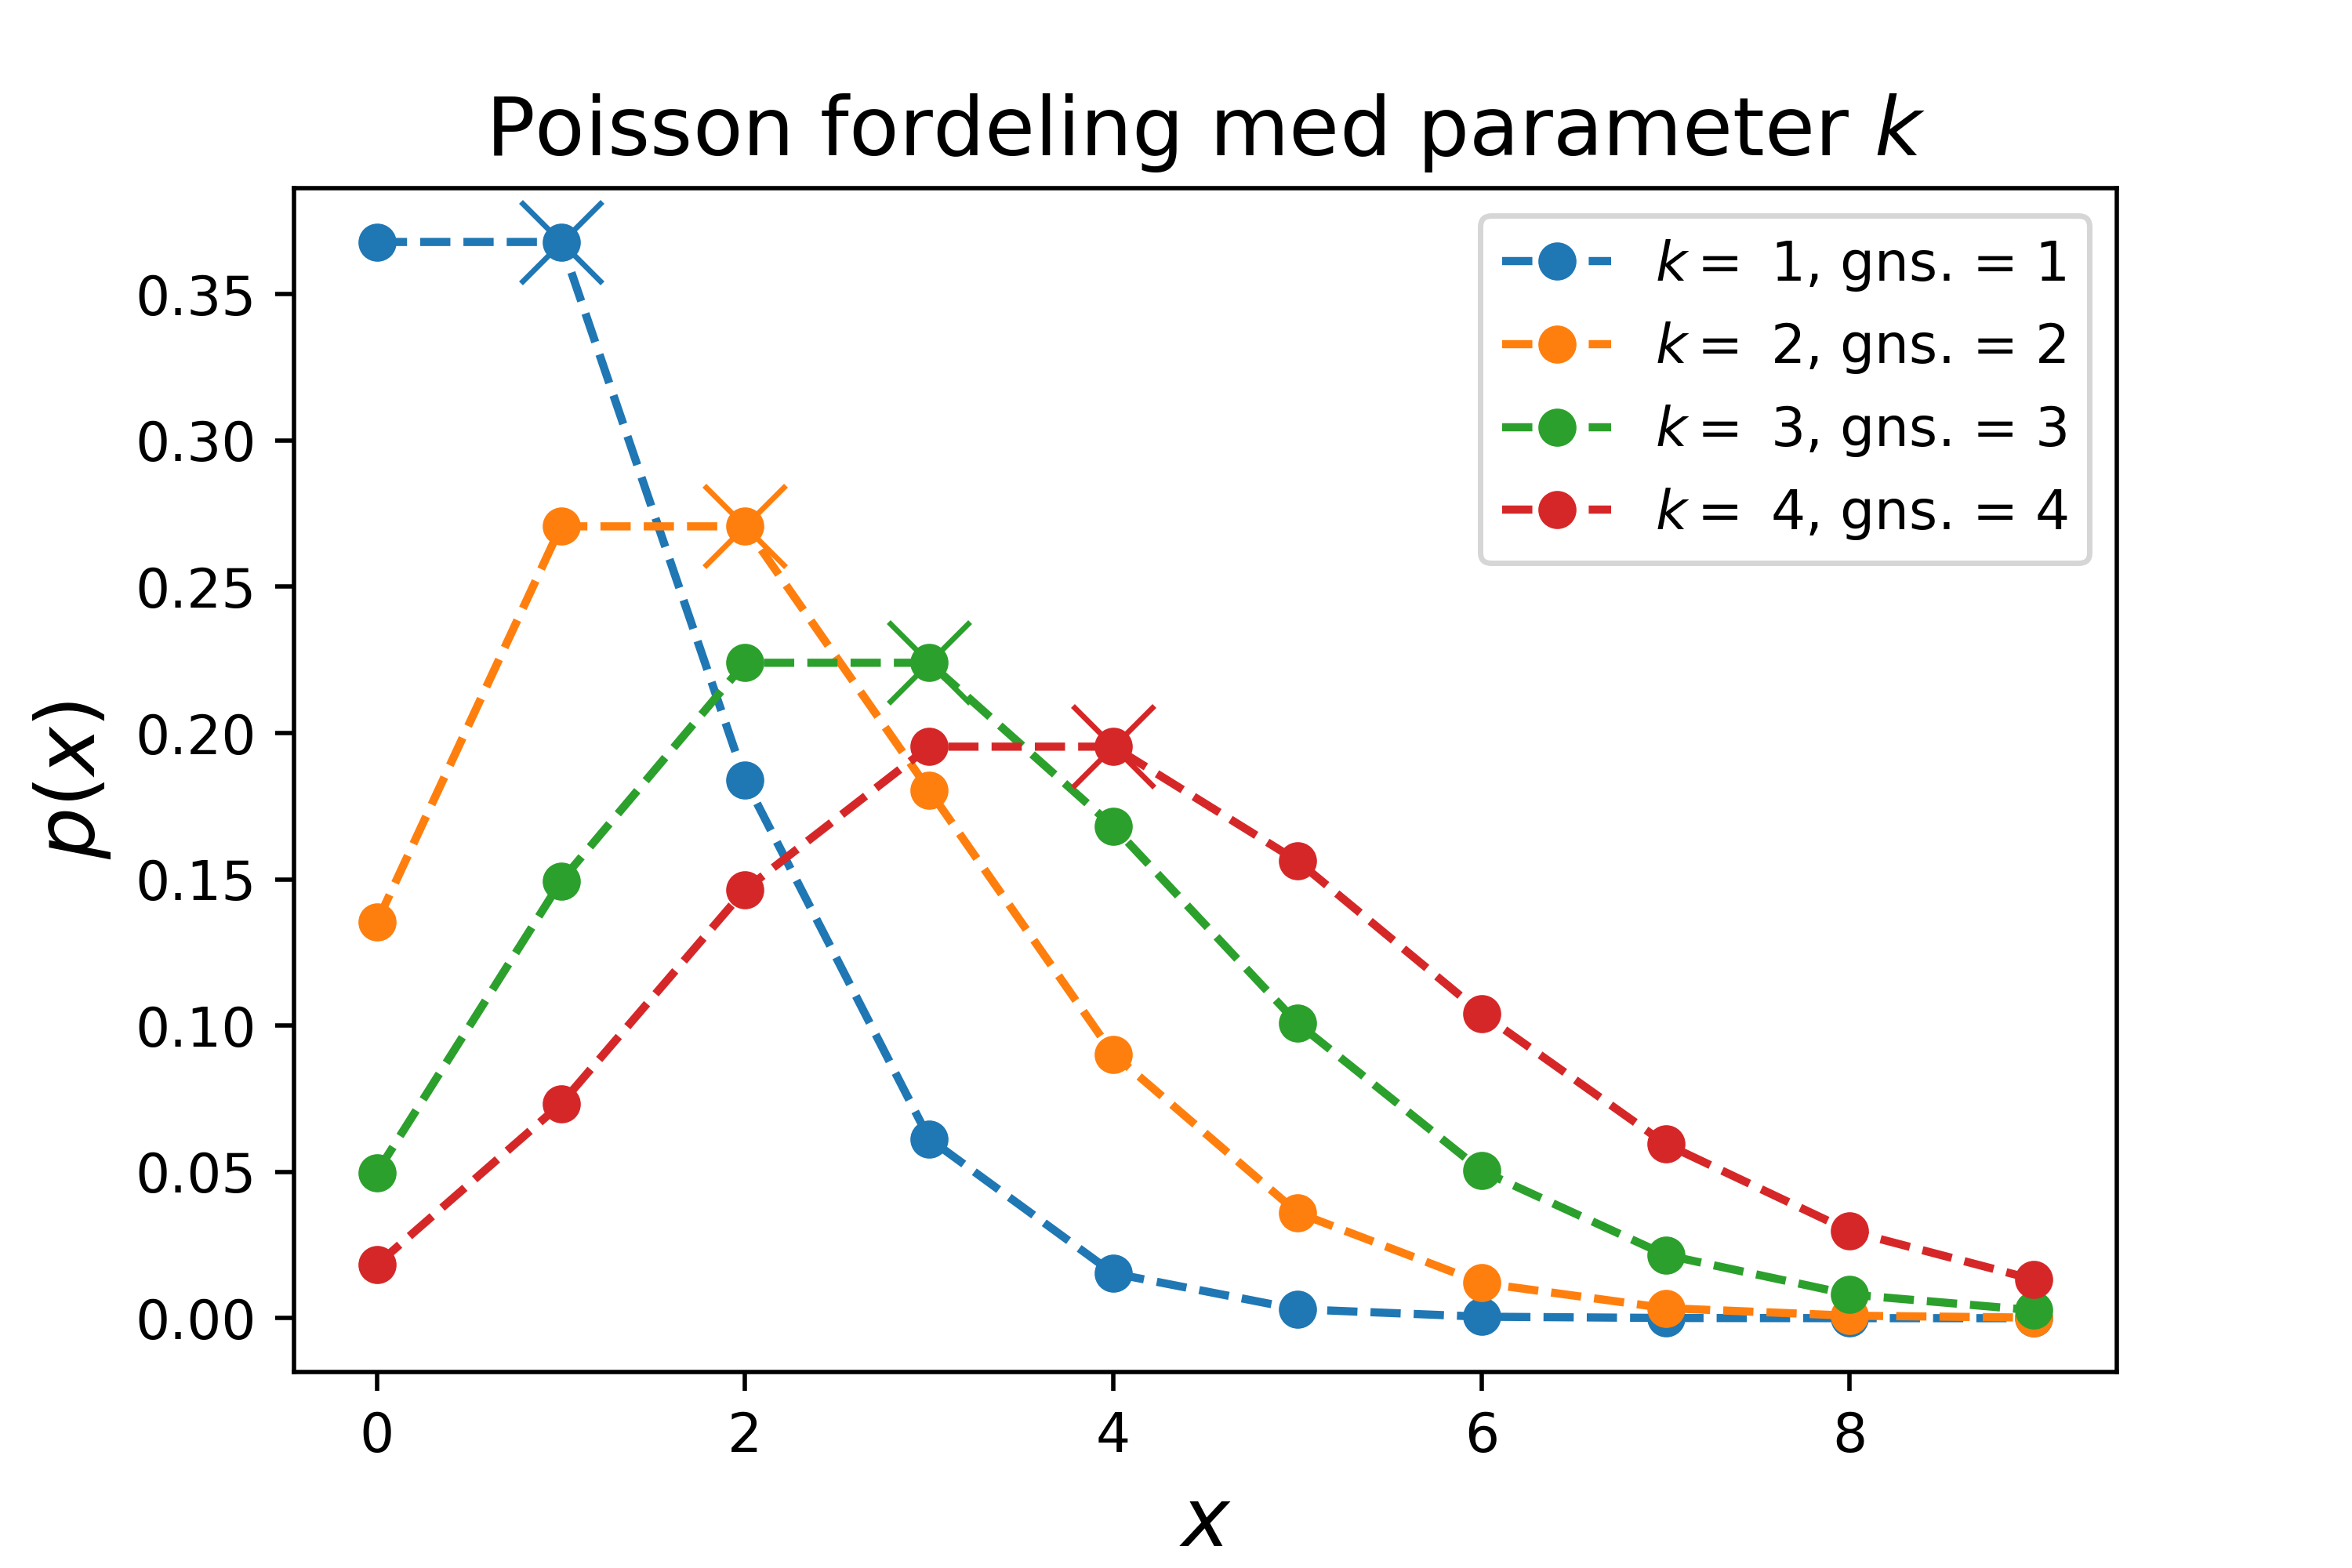
\includegraphics[width = \textwidth]{poiss_dist.png}
\caption{Poisson fordeling med forskellige parmetre $\lambda$. Stjernerne markerer forventet værdi.} \label{fig:poiss}
\end{minipage}
\begin{minipage}[b][][b]{.45\textwidth}
\centering
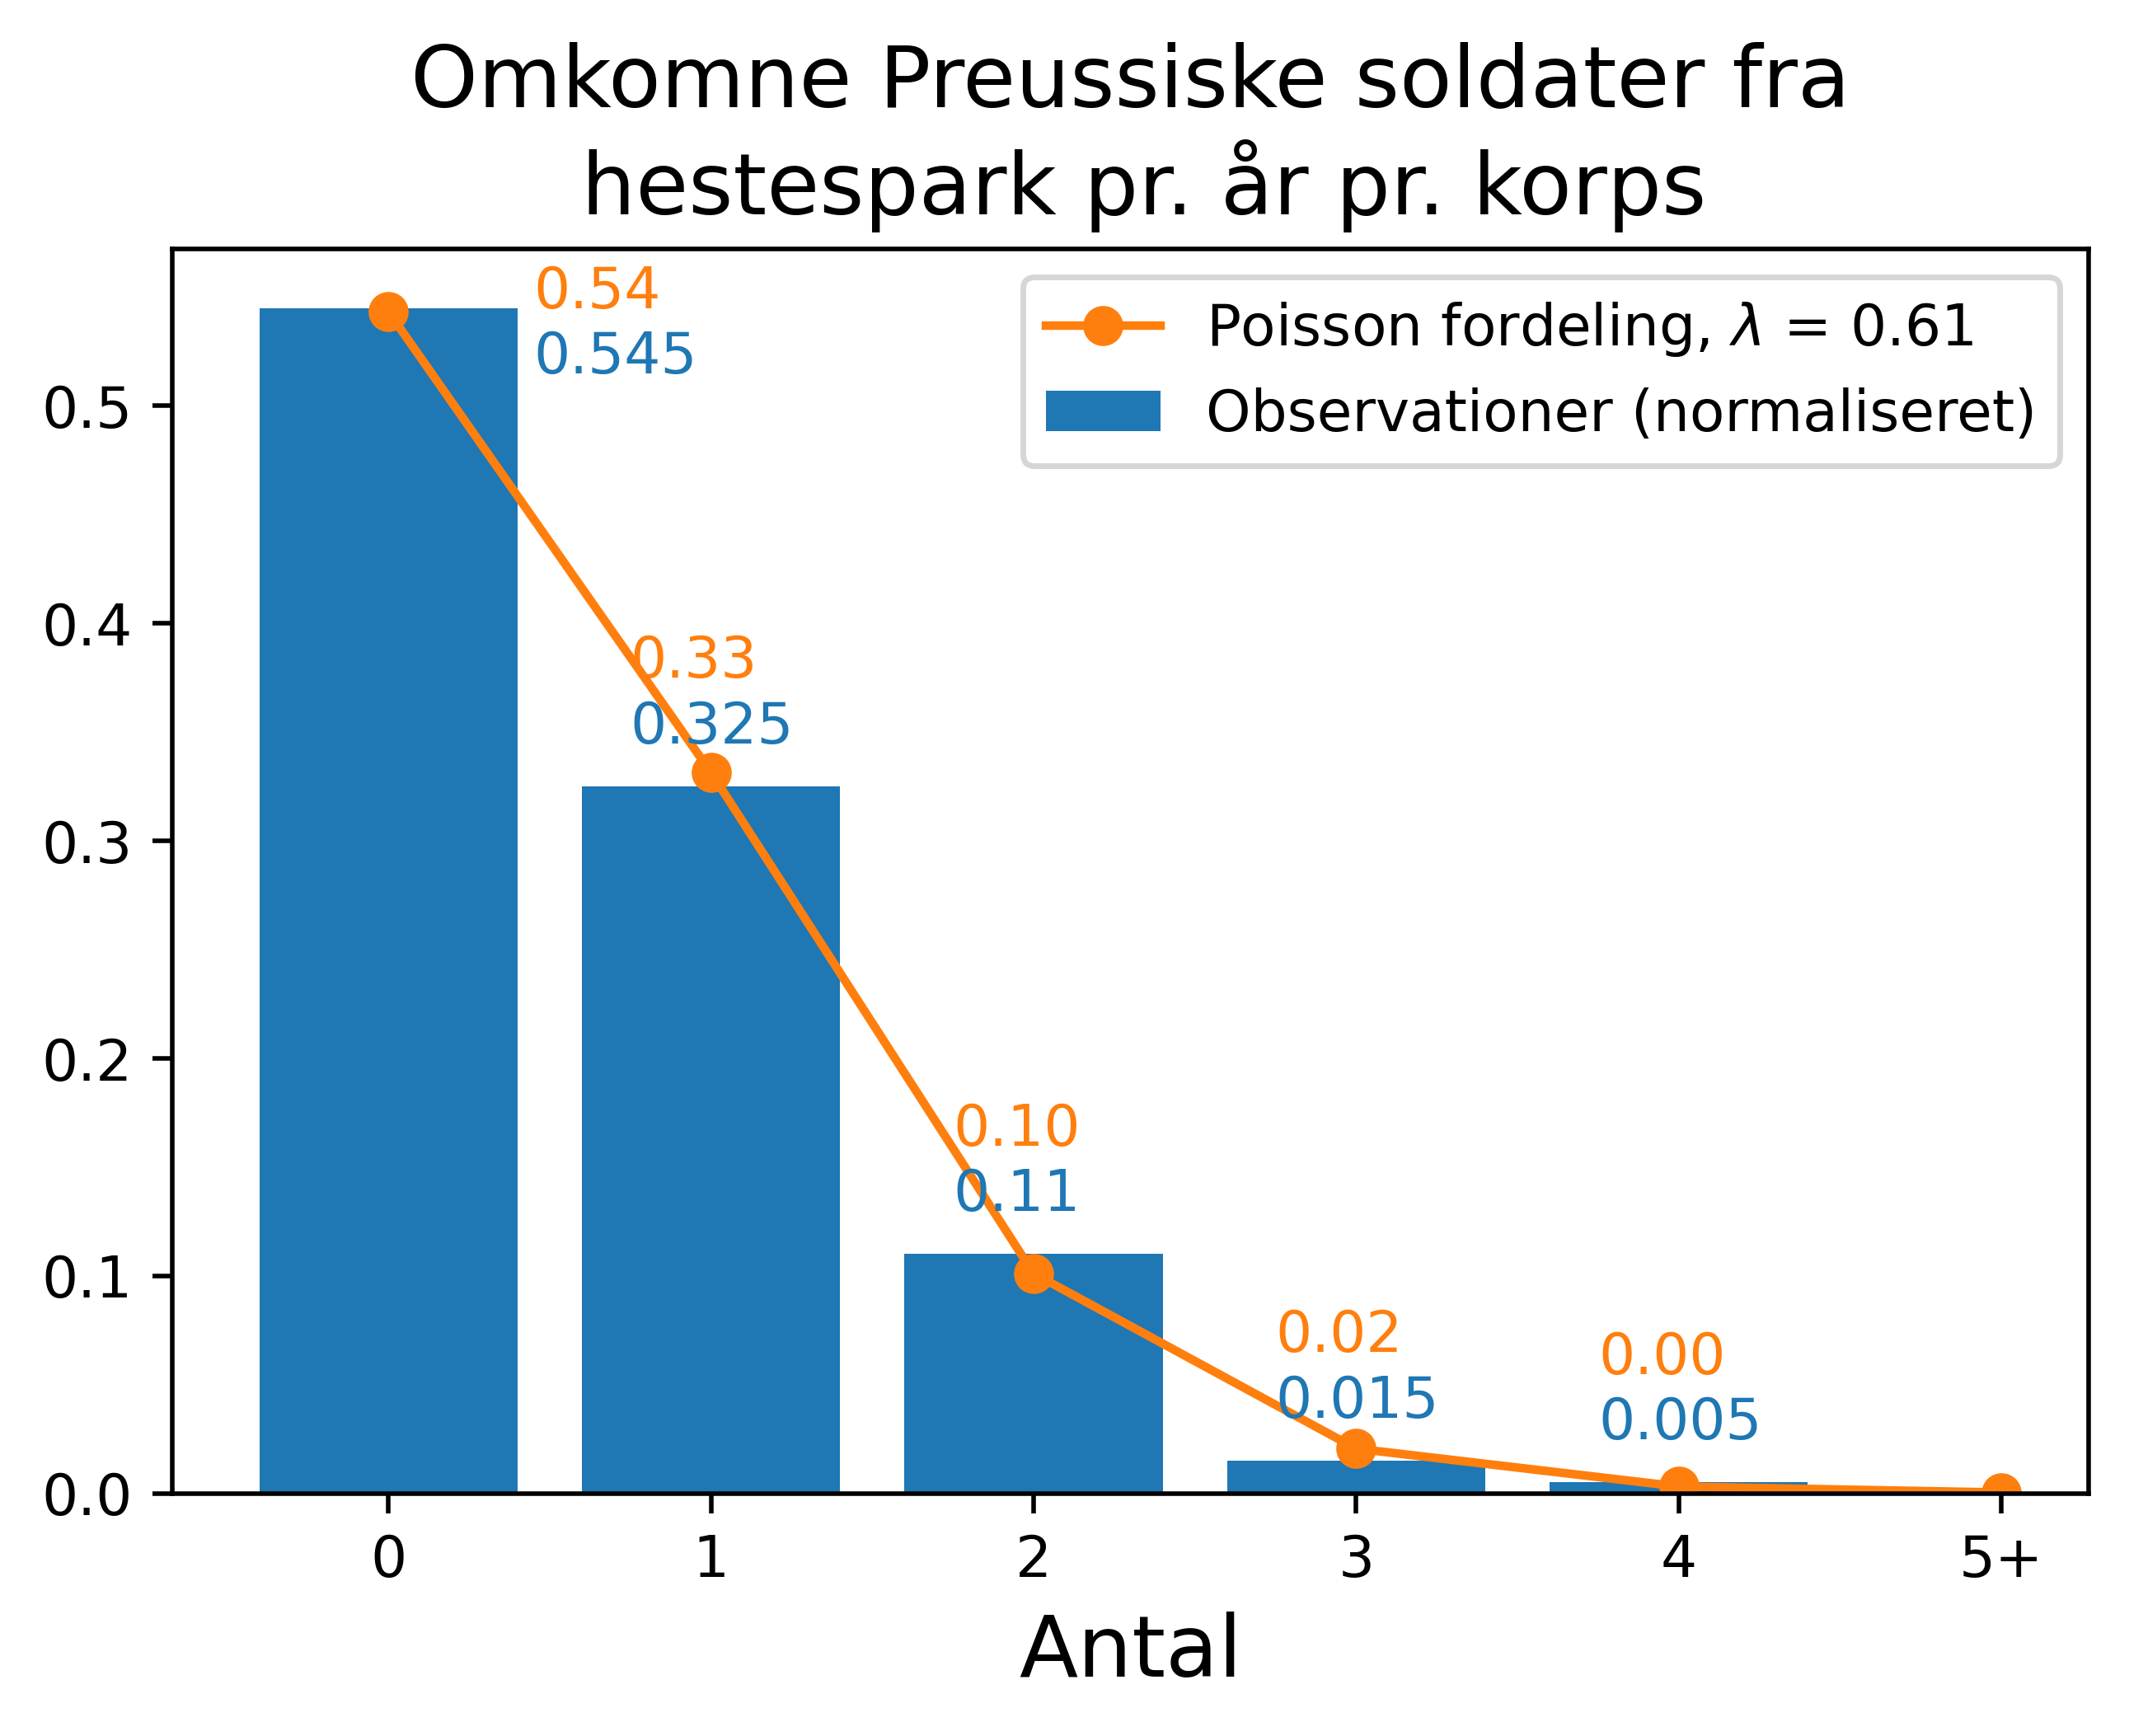
\includegraphics[width = \textwidth]{poiss_example.png}
\caption{Data: \cite{horse}\\ {\color{white}.}} \label{fig:horse}
\end{minipage}
\end{figure}
\subsection{Eksponentielfordeling}
Eksponentielfordelingen er en kontinuert fordeling, som også er vigtig inden for simulering, da den kan bruges til at modellere tiden mellem tilfældige hændelser. Dette kan være jordskælv, ankomst af kunder i en butik og antal tegn inden næste stavefejl i en P1 rapport. Eksponentielfordelingen har egenskaben at være \emph{hukommelsesløs}. Hukommelsesløse tilfældige variable \emph{ældes ikke} i den forstand at sandsynligheden for overlevelse endnu et stykke tid ikke afhænger af nuværende alder. Formelt skrives den hukommelsesløse egenskab for en tilfældig variabel $X$ som: 
\begin{align*}
P(X > x + y \text{ givet } X > y) = P(X > x)
\end{align*}
\begin{example} \label{ex:car1}
I et vejkryds på landet ankommer der en bil en gang i timen gennemsnitligt. Dette vil være en hukommelsesløs process da sandsynligheden for at der ikke kommer en ny bil efter eksempelvis $20$ minutter givet at der ikke er kommet en bil de første $10$ minutter er det samme som sandsynligheden for at der ikke kommer en ny bil efter $10$ minutter. 
\end{example}
Det viser sig at tilfældige variable med den hukommelsesløse egenskab nødvendigvis følger eksponentielfordelingen. Hvis $X$ følger en eksponentielfordeling med parameter $\lambda$ da er pdf'en:
\begin{align*}
p_X(x) = \lambda e^{-\lambda x}, \quad x \geq 0,
\end{align*}
og vi skriver $X \sim \exp(\lambda)$ (se figur \ref{fig:expnorm}). Vi har $E[X] = 1/\lambda$ og $\Var[X] = 1/\lambda^2$, som giver en fortolkning for $\lambda$ der kan refereres til som \emph{fejlraten}. Se \cite[123-127]{olofsson2012} for mere om eksponentielfordelingen. 
\begin{example} \label{ex:car2}
Hvis $T$ måler tiden i sekunder (s) mellem ankomsten af biler i eksempel \ref{ex:car1}, da vil $T$ modelleres godt som en eksponentielfordeling med parameter $\lambda = 1/60^2$ s$^{-1}$ og vi skriver $T \sim \exp(1/60^{2} \text{ s}^{-1})$. 
\end{example}
Den vågne læser har måske bemærket at der er en sammenhæng mellem eksponentielfordelingen, der modellerer tiden mellem tilfældige hændelser, og Poisson fordelingen der måler antallet af tilfældige hændelser inden for en tidsperiode. Denne sammenhæng vil blive belyst i afsnit \ref{sec:pointprocess}. 
\begin{figure}
\centering
\begin{minipage}[b][][b]{.45\textwidth}
\centering
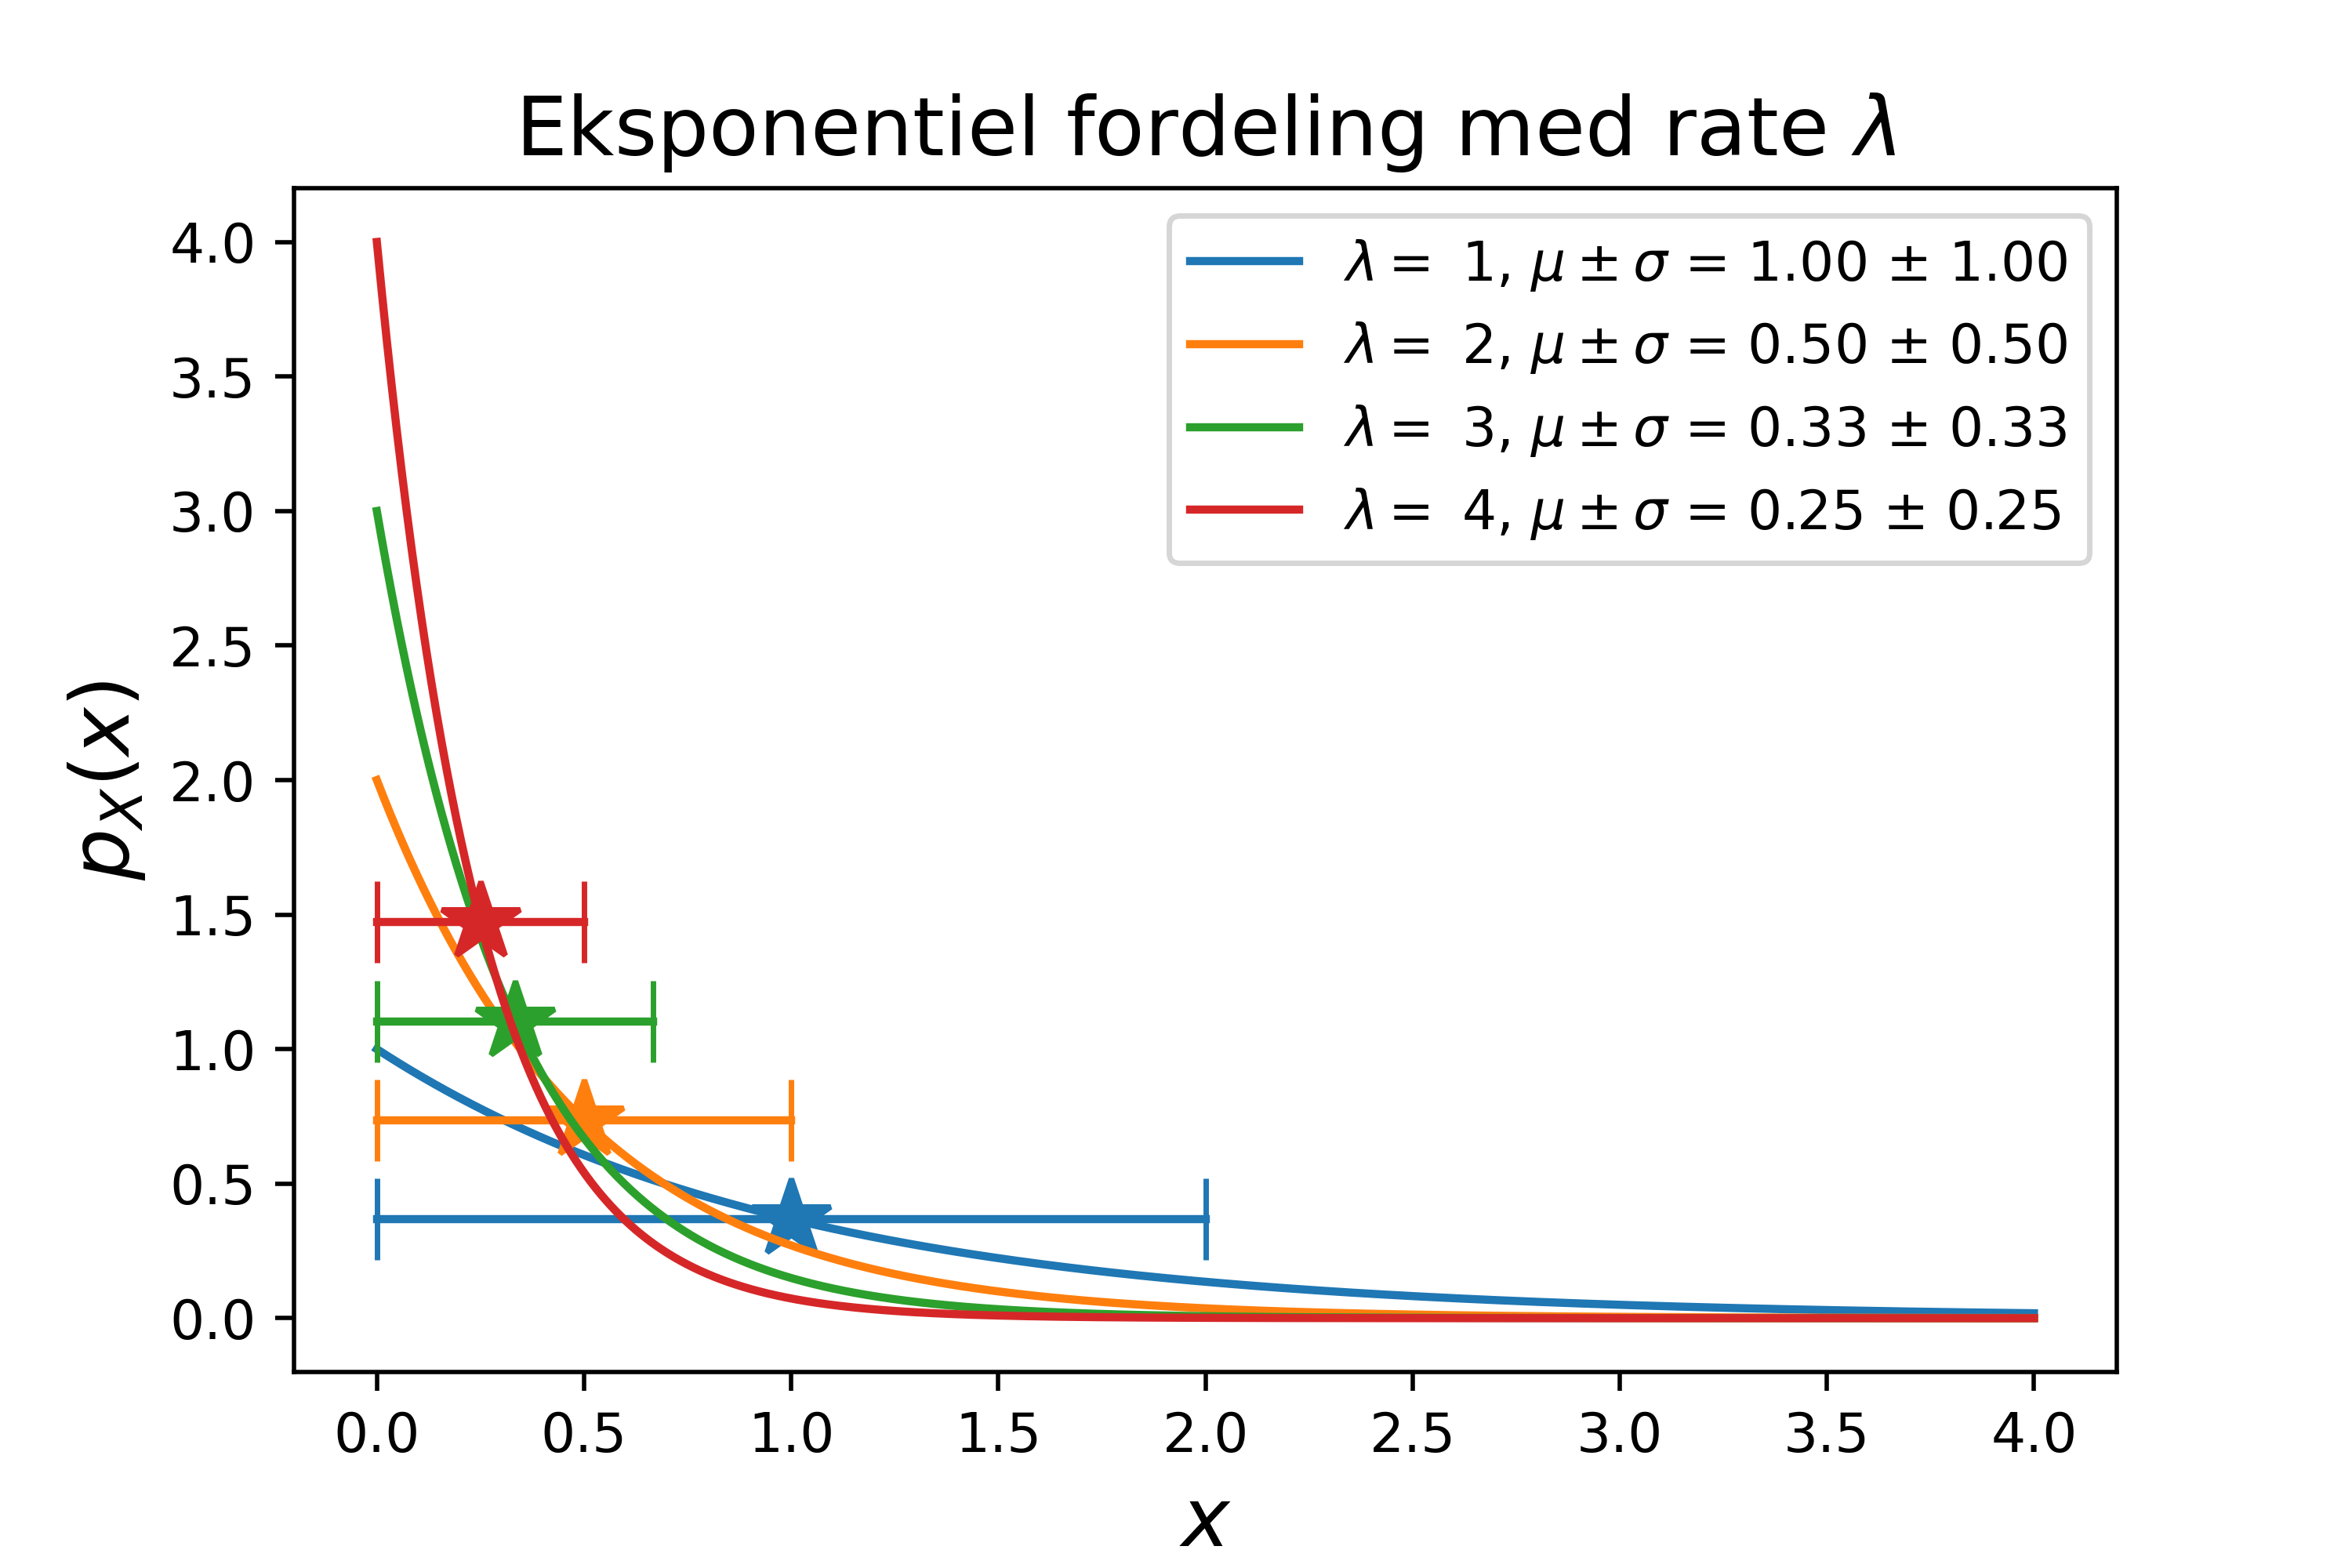
\includegraphics[width = \textwidth]{exp_dist.png}
\end{minipage}
\begin{minipage}[b][][b]{.45\textwidth}
\centering
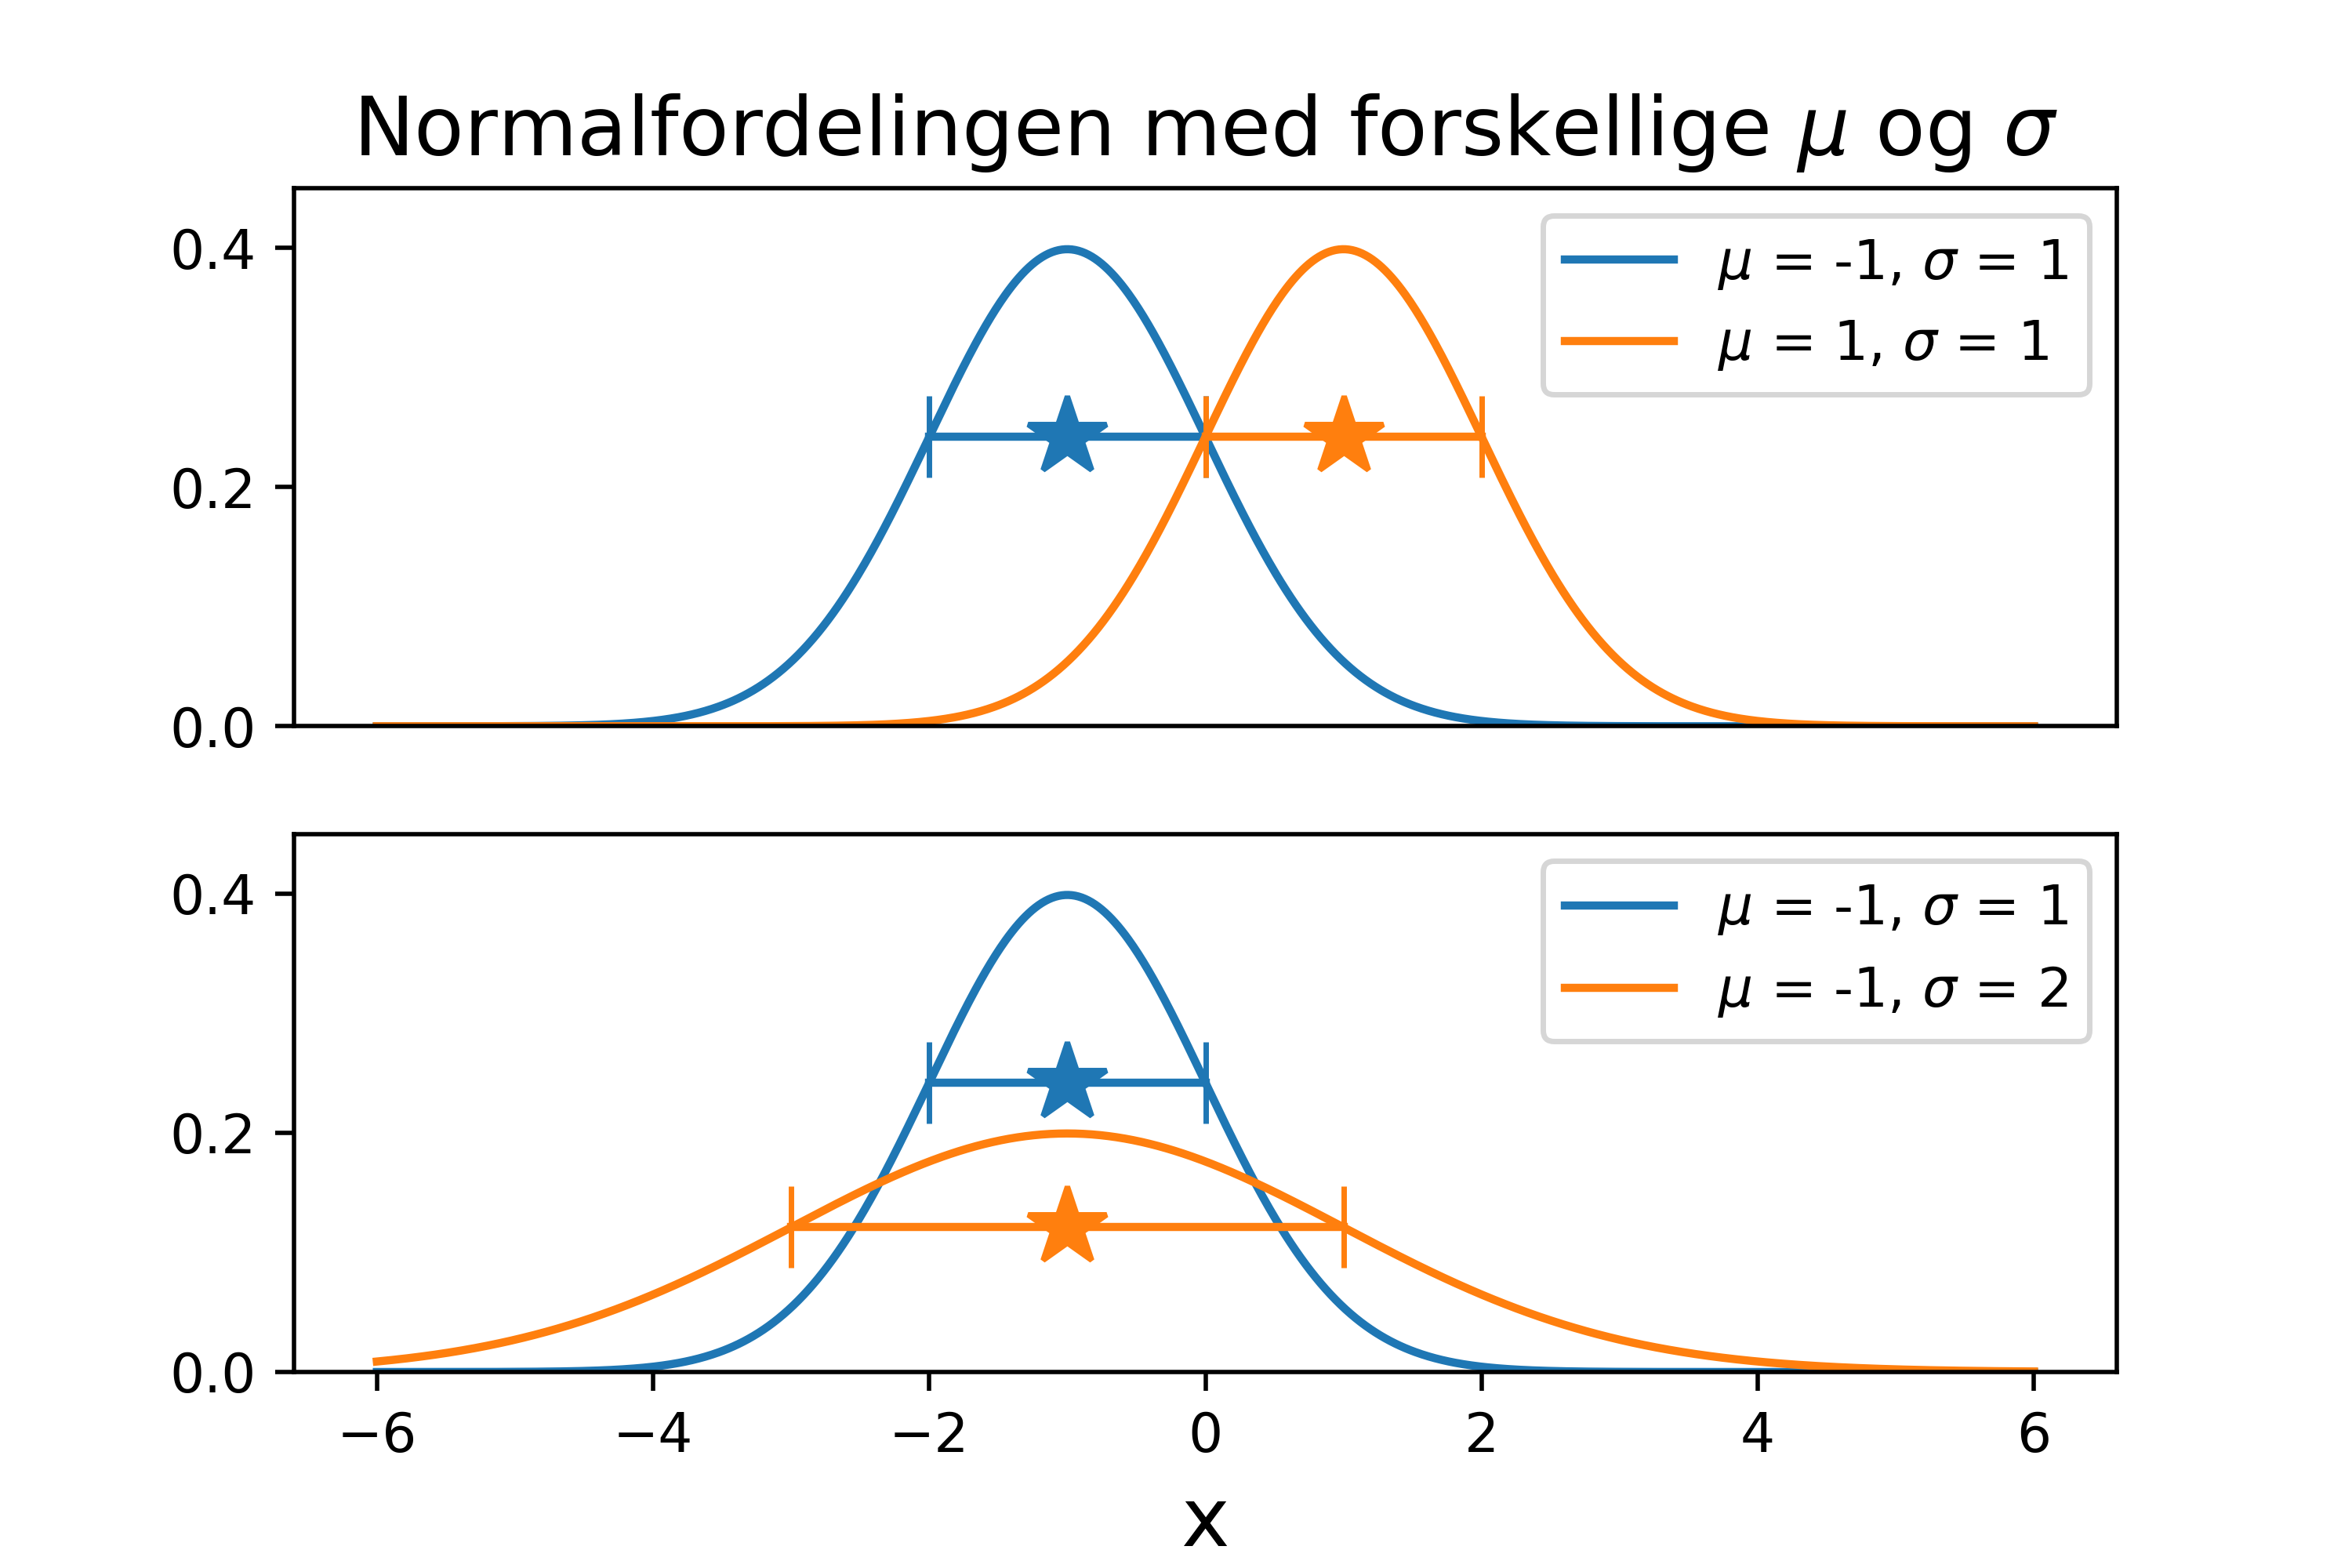
\includegraphics[width = \textwidth]{normal.png}
\end{minipage}
\caption{Eksponentiel og normal fordeling med forskellige parametre. Stjernerne og tilhørende intervaller er forventet værdi $\mu$ $\pm$ standardafvigelse $\sigma$.} \label{fig:expnorm}
\end{figure}
\subsection{Normalfordeling}
Sidst men ikke mindst har vi normalfordelingen. Normalfordelingen er en kontinuert tilfældig variabel, og er den mest brugte indenfor statistik. Den optræder eksempelvis ved støjen på en radiokanal, IQ for en befolkning, spændingen fra en strømforsyning og meget mere. Hvis man ikke kender til fordelingen for en tilfældig variabel vil statistikere ofte antage en normalfordeling.   Fordelingen opstår når der måles en størrelse hvor mange tilfældige faktorer og støj påvirker målingen. Fordelingen er karakteriseret ud fra dens forventede værdi $\mu$ og varians $\sigma^2$, og hvis $X$ følger en normalfordeling med $E[X] = \mu$ og $\Var[X] = \sigma^2$, da er pdf'en:
\begin{align*}
p_X(x) = \frac{1}{\sqrt{2\pi\sigma^2}}\cdot e^{\displaystyle-\frac{1}{2\sigma^2}(x-\mu)^2}, \quad  x \in \mR,
\end{align*}
og vi skriver $X \sim \mathcal{N}(\mu,\sigma^2)$. Se figur \ref{fig:expnorm} for hvordan $\mu$ og $\sigma^2$ har indflydelse på formen på pdf'en. Bemærk at normalfordelingen kan antage alle reelle tal $\mR$. En process hvor negative tal ikke er mulige, såsom vindhastighed, er derfor ikke altid godt modeleret med normalfordelingen især hvis den forventede værdi er tæt på $0$. Se \cite[127-131]{olofsson2012} for mere om normalfordelingen. 

\section{Punktprocesser}
I eksempel \ref{ex:car2} med trafikken i et vejkryds blev tiden mellem to bilers ankomst modelleret med en eksponentielfordelt tilfældig variabel $T$ med parametren $\lambda = 1/60^2$ s$^{-1}$. Lad nu $T_1, T_2, \dots$ være forskellige tilfældige variable der modellerer tiden mellem hver bil over en tidsperiode, eksempelvis en dag, således $T_i \sim \exp(\lambda)$ for $i = 0,1,\dots$. Ankomsttidspunkter over en hel dag er da en såkaldt \emph{punkt process}, hvor hvert punkt markerer ankomstentidspunktet for en bil (se figur \ref{fig:process1}).
\begin{figure}[H]
\centering
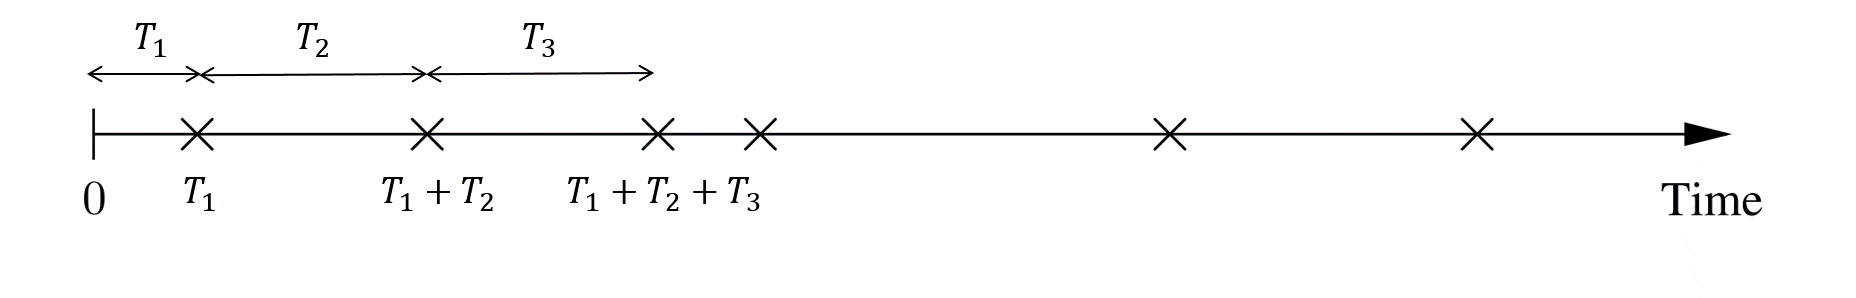
\includegraphics[width = \textwidth]{process1.png}
\caption{Punktprocess hvor $\times$ markerer hændelser i tid, eksempelvis ankomsttidspunkter af biler i et trafikkryds.} \label{fig:process1}
\end{figure}
I det specielle tilfælde hvor $T_1, T_2, \dots$ er eksponentielfordelte med parameter $\lambda$, da er punkt processen den såkaldte \emph{Poisson process}. Poisson processen er nytting til at modellere processer hvor ankomster i tid sker tilfældigt og uafhængigt i tid. Andre eksempler kunne være ankomst af opgaver til en computerserver, kø på apoteket, tidspunkter for jordskælv, ulykker på motervej og henfald af radioaktive partikler.
\\ \\  
Følgende resultat om Possion processer er nyttigt og giver den sammenhæng vi tidligere så mellem Possion og eksponentiel fordelingen. Lad $X(t)$ være en tilfældig variabel der tæller antallet af punkter fra $0$ til $t$ i en Poisson process med parameter $\lambda$. Det viser sig da at $X(t)$ følger en Possion fordeling med parameteren $t \lambda $. Den forventede værdi af $X(t)$ er dermed $E[X(t)] = t \lambda$. $\lambda$ kan således tolkes som antal forventede hændelser per tidsenhed og kaldes af denne grund \emph{raten}. 
\begin{example}
I en lufthavn ankommer hvert døgn gennemsnitligt $400$ fly. Flyene ankommer tilfældigt i løbet af døgnet og er ikke koordineret flyene imellem. Ud fra disse oplysninger kan vi antage en Poisson process for ankomsttidspunkter. Hvis $X(t)$ er antallet af fly i løbet af t timer vil denne følge en Poisson fordeling hvor:
\begin{align*}
E[X(24)] = 24\lambda = 400 \Rightarrow \lambda = 400/24 \approx 16.7,
\end{align*}
således $X(t) \sim \text{Poi}(16.7\cdot t)$ og $T_i \sim \exp(16.7)$. Da tiden mellem to flyvere $T_i$ er eksponentielfordelt med parameter $16.7$ da vil den forventede tid være $E[T_i] = 1/16.7 = 0.06$ timer $= 3.6$ minutter med en standardafvigelse også på $3.6$ minutter. 
\end{example}
Et andet nyttigt resultat kan bruges til nemt at simulere en Poisson process. Vi har givet en Poisson process med rate $\lambda$. Givet at der er $N$ antal punkter i tidsperioden $[0,t]$ vil fordelingen for tidspunkterne være uafhængigt uniformt fordelte tilfældige variable i intervallet $[0,t]$. Kender vi $N$ kan man altså blot simulere $N$ punkter uniformt fordelt i intervallet $[0,t]$ for at simulere en Poisson process. De to resultater om Poisson processen kan således bruges til at simulere dem, hvilket er opsummeret i algoritme \ref{alg:poisprocss}. Se \cite[240-247]{olofsson2012} for mere om Poisson processer. 
\begin{algorithm}
\begin{algorithmic}
\STATE Simuler $N \sim \text{Poi}(t\lambda)$ 
\FOR{$i = 0$ til $N-1$}
\STATE Simuler $Y_i \sim \text{unif}(0,t)$ \COMMENT{$Y_i$ er tidspunktet for en hændelse}
\ENDFOR 
\end{algorithmic}
\caption{Simulering af Poisson process med rate $\lambda$ mellem $0$ og $t$} \label{alg:poisprocss}
\end{algorithm}

\section{Generation af tilfældige tal i C}

\printbibliography[heading=bibintoc]
\label{bib:mybiblio}
\end{document}